% !TEX root = main.tex

%% ─────────────────────────────────────────────────────────────
%% HOW TO ADD A NEW SECTION
%% ─────────────────────────────────────────────────────────────
%% 1. Create:  sections/NN_slug.tex
%%             where NN  = zero-padded number (e.g. 08, 09, 10)
%%             where slug = lowercase-hyphenated section name
%%             e.g.  sections/08_resultados.tex
%%
%% 2. Start the file with:
%%       % [Section name in Portuguese]
%%       \section{Nome da Seção}
%%
%% 3. Add to main.tex (before % Impressão das referências — biblatex
\printbibliography
):
%%       \input{sections/08_resultados}
%%
%% 4. Run:  latexmk -pdf main.tex
%%          (biblatex needs two passes — latexmk handles this automatically)
%% ─────────────────────────────────────────────────────────────

\documentclass[10pt, conference, compsocconf]{IEEEtran}

% --- Encoding & Language ---
\usepackage[utf8]{inputenc}
\usepackage[T1]{fontenc}
\IfFileExists{brazil.ldf}{%
  \usepackage[brazilian]{babel}%
}{%
  \IfFileExists{portuguese.ldf}{%
    \usepackage[portuguese]{babel}%
  }{%
    % Fallback for TeX installations without Portuguese hyphenation patterns.
    % This avoids incorrect English-based syllable breaks in Portuguese words.
    \usepackage[none]{hyphenat}
    \emergencystretch=1em
  }%
}
\usepackage{microtype}

% --- Graphics & Floats ---
\usepackage{graphicx,url}
\usepackage{placeins}

% --- Mathematics ---
\usepackage{amsmath}

% --- Color & Listings ---
\usepackage{xcolor}
\usepackage{listings}

% --- Bibliography (biblatex — UFN style) ---
\usepackage{csquotes} % required by biblatex when babel is loaded
\usepackage[natbib=true, style=numeric, sorting=none, backend=bibtex]{biblatex}
\addbibresource{references.bib}

% --- Hyphenation exceptions ---
\hyphenation{op-tical net-works semi-conduc-tor}


\begin{document}

% Título e bloco de autores — UFN IEEEtran
\title{Alchemon: O Uso de Mecânicas de \textit{Creature Capture} e Aprendizagem Tangencial no Ensino da Tabela Periódica}

\author{\IEEEauthorblockN{Mateus Nedel dos Reis, Iuri Lammel Marques}
\IEEEauthorblockA{Curso de Jogos Digitais\\
UFN - Universidade Franciscana\\
Santa Maria - RS\\
m.nedel@ufn.edu.br,
orientador@ufn.edu.br}
}

\maketitle
% Resumo e palavras-chave no formato UFN
\begin{abstract}
A disciplina de Química no Ensino Médio, particularmente no que diz respeito à Tabela Periódica, enfrenta desafios críticos devido ao excesso de abstração e ao baixo engajamento dos estudantes. O objetivo principal deste projeto é desenvolver o Alchemon, um jogo sério que utiliza mecânicas de captura e colecionismo de criaturas para promover a aprendizagem tangencial e o engajamento volitivo dos estudantes. A base teórica baseia-se na fusão da Teoria da Autodeterminação, da Teoria da Aprendizagem Significativa e da Aprendizagem Tangencial, combinadas com a Taxonomia de Bloom para concentrar a carga cognitiva nos alunos. Os resultados deste trabalho demonstram a viabilidade técnica da proposta, validam o enquadramento conceitual e o cronograma necessários para o futuro desenvolvimento e validação prática do protótipo.
\end{abstract}

\textbf{\textit{Palavras-chave}: jogo sério; ensino de Química; aprendizagem tangencial; \textit{Game-Based Learning}; Tabela Periódica.}

\IEEEpeerreviewmaketitle
\section{INTRODUÇÃO}
A sociedade contemporânea vivencia uma fase de transformações profundas no campo educacional, em que o ensino tradicional enfrenta o desafio de se adaptar às novas linguagens e dinâmicas da era digital \cite{Bellotti2010}.
Nesse cenário, a inserção das Tecnologias de Informação e Comunicação (TICs) e, especificamente, do \textit{Game-Based Learning} (GBL), tem se consolidado como uma estratégia de mediação pedagógica eficaz para aumentar o engajamento discente \cite{Turkay2012}.
Os jogos digitais, ao integrarem elementos lúdicos a objetivos de instrução, deixaram de ser meros artefatos de entretenimento para se tornarem ambientes complexos de construção de conhecimento e desenvolvimento de habilidades críticas \cite{Soriano-Sanchez2026}.
Essa evolução tecnológica permite criar contextos situados onde o aprendizado ocorre imersivamente, assim supera as limitações de modelos puramente expositivos e proporciona experiências que favorecem a retenção de informações a longo prazo \cite{Bellotti2010,Espirito2020}.

Contudo, a despeito do potencial das novas tecnologias, os índices de desempenho escolar em áreas fundamentais permanecem em patamares alarmantes.
No âmbito das ciências da natureza, o relatório do PISA 2022 revela um déficit quantitativo significativo no sistema educacional brasileiro, no qual a pontuação média em ciências fixou-se em 403 pontos, valor substancialmente abaixo da média da OCDE, de 485 pontos.
De forma mais crítica, os dados estatísticos indicam que apenas cerca de 45\% dos estudantes brasileiros atingiram o nível mínimo de proficiência em ciências (Nível 2). 
Isso implica que a maioria absoluta dos jovens não consegue reconhecer explicações corretas para fenômenos científicos familiares ou identificar se uma conclusão é válida com base em dados simples, reflete uma estagnação no letramento científico que persiste há mais de uma década \cite{OECD2023}.

Este déficit de aprendizagem é particularmente acentuado no ensino de Química, disciplina frequentemente percebida pelos estudantes como um domínio de excessiva abstração e complexidade \cite{Latonio2023,Lackey2022}. 
O estudo de tópicos fundantes, como a Atomística e a Tabela Periódica, é marcado por uma aversão histórica por parte dos alunos, frequentemente agravada por práticas pedagógicas que priorizam a recepção passiva e a memorização mecânica de símbolos, fórmulas e tendências periódicas. 
Tais métodos tradicionais resultam em sobrecarga cognitiva e falham ao tentar estabelecer conexões entre as estruturas microscópicas e os fenômenos do cotidiano, e gera uma fragmentação do conhecimento.
A frustração das necessidades psicológicas básicas de autonomia e competência dos estudantes culmina em um cenário de baixo engajamento e desinteresse pela continuidade dos estudos na área \cite{Lima2010}.
Diante dessa conjuntura, manifesta-se uma necessidade latente de ferramentas lúdicas e interativas que realizem a transposição didática de conceitos químicos para sistemas digitais integrados, capazes de preencher essa lacuna pedagógica e transformar o esforço intelectual em um processo volitivo e significativo \cite{Han2021,Latonio2023}.

Nesta seção, define-se os objetivos do projeto, justifica-se a escolha de jogos sérios como solução pedagógica e apresenta-se a delimitação do problema.

\subsection{Objetivo geral}
Desenvolver o jogo sério Alchemon, por meio de mecânicas de captura e colecionismo de criaturas como estratégia para promover a aprendizagem tangencial e o engajamento volitivo de estudantes do Ensino Médio no domínio da Tabela Periódica.

\subsection{Objetivos específicos}
Para a consecução do objetivo geral e o desenvolvimento do jogo sério Alchemon, estabelecem-se os seguintes objetivos específicos:
\begin{itemize}
    \item Investigar o estado da arte e as fragilidades no ensino de Química para o Ensino Médio, correlacionando-as aos referenciais de engajamento volitivo da Teoria da Autodeterminação (SDT) e da Aprendizagem Significativa (TAS);
    \item Mapear as propriedades físico-químicas e tendências periódicas dos elementos químicos para a transposição didática em arquétipos e atributos de criaturas colecionáveis;
    \item Projetar a arquitetura do jogo por meio de um \textit{Game Design Document} (GDD), definir mecânicas de captura e colecionismo que operem como organizadores prévios alinhados aos níveis de \enquote{Lembrar} e \enquote{Entender} da Taxonomia de Bloom;
    \item Desenvolver o protótipo funcional do jogo em um motor de jogos, como Unity ou Godot, programar sistemas de \textit{feedback} imediato e ciclos de maestria para satisfazer a necessidade de competência do jogador;
    \item Implementar ferramentas de aprendizagem tangencial, como enciclopédias \textit{in-game} e espaços informativos, visando estimular a pesquisa autodidata sobre o conteúdo científico fora do ambiente virtual.
\end{itemize}

\subsection{Justificativa}
O ensino de Química no Ensino Médio, particularmente no que tange ao domínio da Tabela Periódica e da atomística, enfrenta desafios críticos relacionados à excessiva abstração dos conteúdos e ao baixo engajamento dos estudantes \cite{Latonio2023}. 
Métodos tradicionais baseados na recepção passiva falham em promover a compreensão das relações entre os níveis macroscópico e microscópico da matéria, o que resulta em uma memorização mecânica que compromete a retenção do conhecimento a longo prazo \cite{Lima2010}.

Dados do PISA \cite{OECD2023} e avaliações nacionais corroboram um cenário de desinteresse generalizado pelas ciências básicas \cite{SilvaFilho2023}. 
Nesse panorama, a Aprendizagem Baseada em Jogos (GBL) \cite{Plass2020} surge como uma ferramenta de intervenção pedagógica necessária, que apresenta um tamanho de efeito superior aos meios convencionais para o ensino de ciências naturais \cite{Soriano-Sanchez2026}.
Os jogos digitais oferecem ambientes imersivos nos quais a cognição situada permite que o aprendizado ocorra dentro de um contexto funcional \cite{Bellotti2010}, que facilitam a transposição didática por meio de desafios progressivos \cite{Li2024}.

\subsection{Delimitação do Estudo}
O presente projeto delimita-se ao planejamento e design instrucional dos conteúdos programáticos iniciais de Química Geral e Físico-Química, convergindo as diretrizes da Base Nacional Comum Curricular (BNCC) para o Ensino Médio \cite{BNCC26} e o referencial internacional \textit{Cambridge IGCSE Chemistry} \cite{igcse_chemistry_2023}. O escopo pedagógico do jogo \textit{Alchemon} compreende especificamente os módulos de: (i) Estados da Matéria e Modelos Atômicos; (ii) Tabela Periódica e Propriedades Periódicas; (iii) Ligações Químicas (Iônica, Covalente e Metálica). 

Estão explicitamente excluídos deste ciclo inicial de desenvolvimento os tópicos avançados de Termoquímica, Cinética, Equilíbrio Químico e Química Orgânica. Essa delimitação justifica-se pela necessidade de consolidar um Produto Mínimo Viável (MVP) que valide a arquitetura lúdico-pedagógica proposta, assegurando a profundidade mecânica necessária para a compreensão das relações estequiométricas antes da expansão para outras áreas da disciplina.

\subsection{Estrutura do trabalho}
Este trabalho está organizado em seis seções principais, estruturadas conforme descrito a seguir:

Na Seção 2, apresenta-se o referencial teórico, abordam-se conceitos da Teoria da Autodeterminação (SDT), da Teoria da Aprendizagem Significativa (TAS), da Aprendizagem Tangencial, da Taxonomia de Bloom e define-se o gênero de Creature Capture.
A Seção 3 detalha-se os trabalhos correlatos, estabelece-se um comparativo entre o projeto Alchemon e outras iniciativas da área.
A Seção 4 descreve a metodologia científica adotada e o planejamento para o desenvolvimento do protótipo.

A Seção 5 dedica-se à identificação e resolução do problema, ao detalhar a aplicação prática dos conceitos pedagógicos no design das mecânicas do jogo.
Por fim, a Seção 6 apresenta as conclusões parciais, bem como as sugestões para o prosseguimento da pesquisa e trabalhos futuros.

\section{REFERENCIAL TEÓRICO}
Neste tópico, apresenta-se o referencial teórico que fundamenta esta pesquisa. Conceituam-se as principais teorias que serviram de fundação para o \textit{game design} e elementos do game design, definição do gênero e de jogos sérios.

\subsection{Teoria da Autodeterminação (SDT) e motivação}
Proposta por Richard Ryan e Edward Deci \cite{Ryan1985}, a Teoria da Autodeterminação (SDT) é uma estrutura organísmica \cite{Ryan2020} que assume que os seres humanos possuem uma propensão inerente para o crescimento e a integração, mas necessitam de suportes ambientais para florescer \cite{Ryan1985}. A teoria postula três necessidades psicológicas fundamentais e universais \cite{Ryan1985}: a autonomia, que compreende o senso de iniciativa e propriedade sobre as ações; a competência, referente ao sentimento de maestria e eficácia; e o relacionamento, que abrange o senso de pertencimento e conexão social \cite{Shi2016}. Como essas necessidades se relacionam com a motivação, pode ser visto na Fig. \ref{fig:sdt}.

\begin{figure}[H]
    \centering
    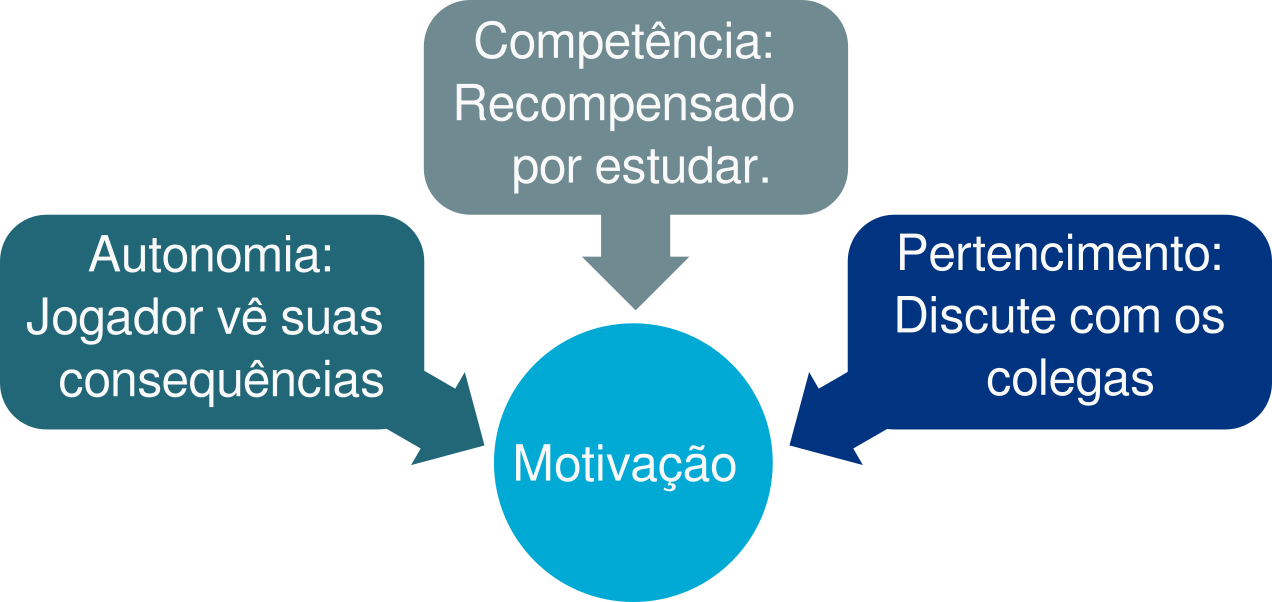
\includegraphics[width=0.4\textwidth]{images/sdt.png}
    \caption{Teoria da Autodeterminação (SDT). Fonte: elaborado pelo autor.}
    \label{fig:sdt}
\end{figure}

Ryan e Deci \cite{Ryan1985} dividem a motivação em dois tipos principais: motivação intrínseca, que é impulsionada por interesses e prazeres inerentes à atividade, e motivação extrínseca, orientada por recompensas ou pressões externas. Nos jogos, a motivação intrínseca é desenvolvida quando o design proporciona ao jogador agência para completar objetivos, além de permitir novas tentativas após falhas (\textit{graceful failure}) e a colaboração com outros jogadores \cite{Plass2020}. A motivação extrínseca, por sua vez, é frequentemente implementada por meio de sistemas de recompensas, como pontos, medalhas e tabelas de classificação \cite{Coelho2025}.

Ao aprofundar a análise da SDT no contexto lúdico, a Teoria da Integração Organísmica (OIT) \cite{Ryan2022} explica como comportamentos inicialmente motivados por fatores externos podem ser internalizados e integrados ao \textit{self}. Para que essa transição ocorra, o ambiente de jogo deve possuir uma significância funcional informacional \cite{Gao2024}, na qual o jogador percebe o \textit{feedback} e as recompensas como suportes à sua competência, e não como mecanismos de controle. 

Estudos indicam que o uso de recompensas pode minar a motivação intrínseca se forem compreendidas como controladoras, por reduzir a autonomia do jogador \cite{Ryan2022}. Inversamente, recompensas intrínsecas, que oferecem novas habilidades ou acesso a conteúdos, reforçam o engajamento volitivo \cite{Ryan2022}, definido como o estado de envolvimento ativo e focado no jogo. Além disso, a satisfação das necessidades é mutuamente informativa, pois a competência só gera motivação de alta qualidade quando acompanhada por um senso de autonomia, permitindo que o jogador sinta-se o \textit{locus} de causalidade de seu sucesso \cite{Ryan1985, Gao2024}.

\subsection{Teoria da Aprendizagem Significativa (TAS) e organizadores prévios}
David Ausubel fundamentou a Aprendizagem Significativa (TAS) \cite{Ausubel1963} no princípio de que novas ideias são assimiladas apenas quando ancoradas em conhecimentos prévios estáveis, processo denominado subsunção \cite{Espirito2020}. Para mitigar o distanciamento entre o que o estudante já sabe e o material novo, Ausubel \cite{Ausubel1963} propôs o uso de organizadores prévios, que são materiais introdutórios apresentados em um nível mais alto de abstração e generalidade. Esses materiais servem como pontes conceituais para destacar a importância do novo conteúdo \cite{Custodio2015}. No \textit{design} de jogos, isso se manifesta em tutoriais que apresentam a estrutura do sistema antes da complexidade total, permitindo a diferenciação progressiva do conhecimento \cite{Espirito2020, Custodio2015}.

Recentes revisões críticas da TAS, fundamentadas em avanços da neurociência, sugerem que a memória não é um constructo estático, mas um processo dinâmico e generativo \cite{Bryce2024}. Sob esta ótica, a aprendizagem significativa não envolve a substituição de concepções intuitivas, conhecidas como alternativas, mas sim um processo de coexistência conceitual e revisão. Nesse processo, o aprendiz desenvolve a habilidade de selecionar o repertório (\textit{scaffolding}), seja ele cotidiano ou científico, mais adequado à situação imediata. Em vez de apenas suportes temporários (\textit{scaffolding}), propõe-se o uso de \textit{cantilevers} conceituais , que são estruturas de apoio permanentes baseadas no conhecimento prévio que sustentam a construção de novos saberes \cite{Bryce2024}. Tal analogia pode ser compreendiada na Fig. \ref{fig:tas}.

\begin{figure}[H]
    \centering
    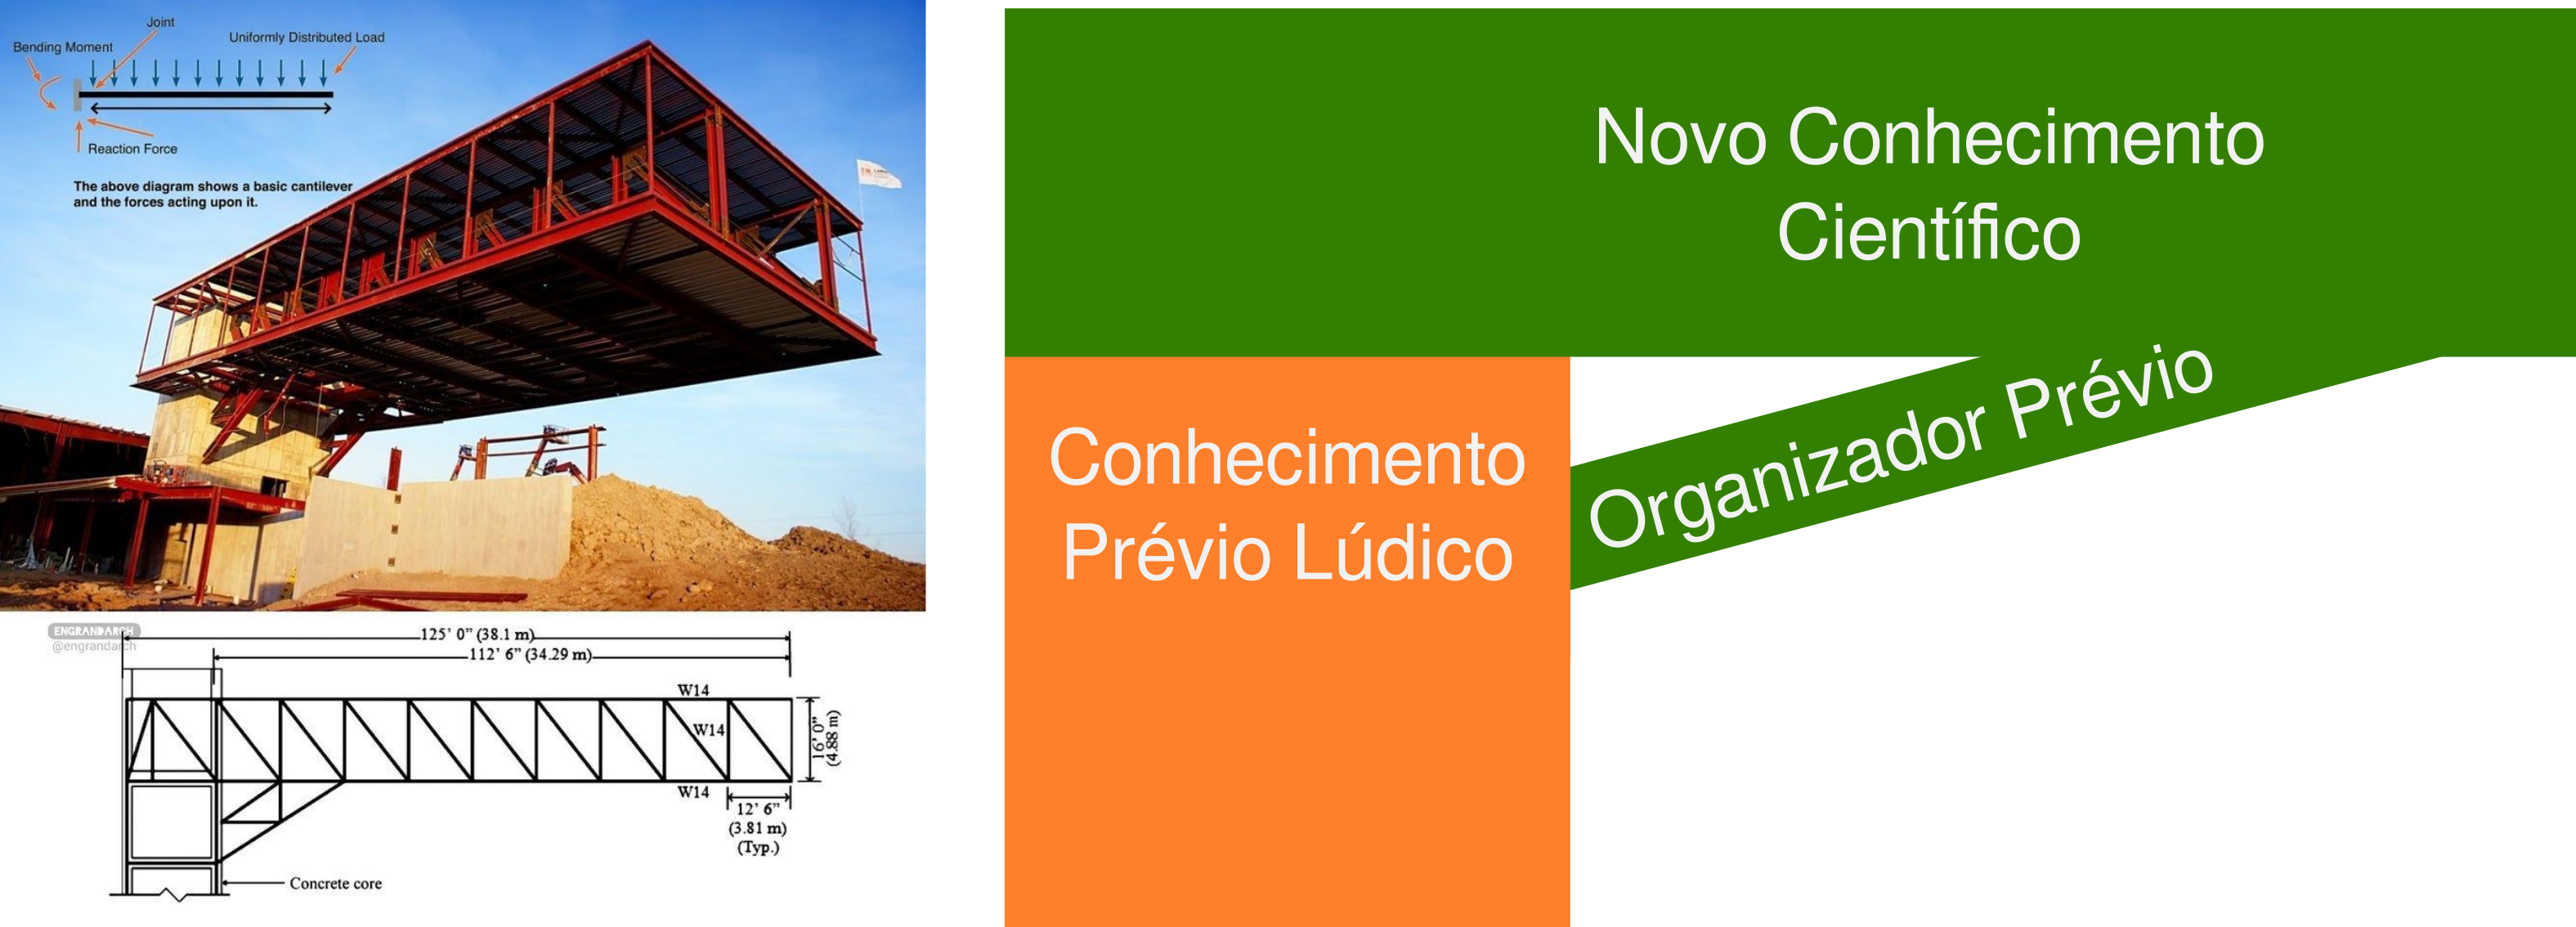
\includegraphics[width=0.4\textwidth]{images/tas.png}
    \caption{Teoria da Aprendizagem Significativa (TAS). Fonte: elaborado pelo autor.}
    \label{fig:tas}
\end{figure}

\subsection{Aprendizagem Tangencial}
A Aprendizagem Tangencial \cite{Portnow2012} refere-se ao processo espontâneo no qual o jogador adquire conhecimentos periféricos ao interagir com mídias de entretenimento que não têm o ensino como objetivo primário \cite{Mozelius2017}. Isso ocorre quando o jogador se envolve com elementos ludo-narrativos \cite{LimadaCostaJunior2022}, a exemplo da história de \textit{Assassin's Creed} ou das mecânicas de química em Batalha Quimicard \cite{GomesdeFreitas2017}, e busca voluntariamente aprofundar esses temas em fontes externas \cite{Lorenzatti2020}. Tal interação pode ser visualizada na Fig. \ref{fig:tangencial}. Designers utilizam ferramentas referenciais como enciclopédias \textit{in-game}, espaços informativos em telas de carregamento com curiosidades e referências diretas a artefatos reais para estimular essa curiosidade \cite{Lorenzatti2020}.

\begin{figure}[H]
    \centering
    
\includegraphics[width=0.4\textwidth]{images/tangencial.png}
    \caption{Aprendizagem Tangencial. Fonte: elaborado pelo autor.}
    \label{fig:tangencial}
\end{figure}

A eficácia desse processo pedagógico está intimamente ligada à integração intrínseca do conteúdo às mecânicas de vitória, a fim de que o objeto de conhecimento constitua a própria natureza do jogo e não um elemento meramente ilustrativo ou uma barreira enfadonha \cite{Mozelius2017}. Estudos indicam que, em jogos nos quais o conhecimento foi integrado com sucesso, as mecânicas servem como plataformas experimentais para que o jogador teste conceitos adquiridos externamente \cite{Mozelius2017}. No jogo sério Batalha Quimicard \cite{GomesdeFreitas2017}, por exemplo, a internalização de constantes como $K_a$ e $K_b$ para formular estratégias de duelo demonstra como o jogador se apropria do conceito científico para obter êxito sistêmico.

\subsection{Taxonomia de Bloom}
A Taxonomia de Bloom \cite{Bloom1956}, sistematizada em 1956 e revisada por Anderson e Krathwohl em 2001 \cite{Anderson2001}, categoriza os processos cognitivos em níveis de complexidade crescente: Lembrar, Compreender, Aplicar, Analisar, Avaliar e Criar. Pode ser compreendida como uma pirâmide, a exemplo da Fig. \ref{fig:bloom}, que inicia com os níveis baixos de Lembrar e Compreender. No design de jogos sérios \cite{Plass2020}, esse \textit{framework} é utilizado para alinhar a mecânica de jogo ao desempenho acadêmico esperado, garantindo que o conteúdo seja introduzido de forma estruturada.

\begin{figure}[H]
    \centering
    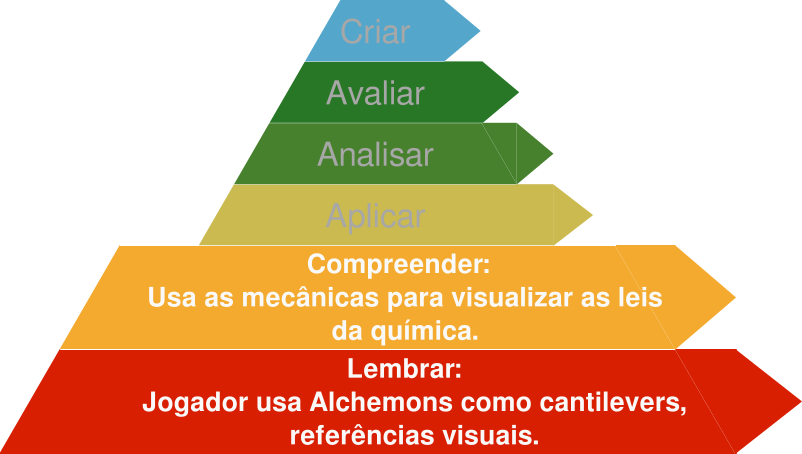
\includegraphics[width=0.4\textwidth]{images/bloom.png}
    \caption{Taxonomia de Bloom. Fonte: elaborado pelo autor.}
    \label{fig:bloom}
\end{figure}

Diferente de abordagens que buscam a maestria total do espectro cognitivo, o Alchemon foca deliberadamente nos níveis de ordem inferior: Lembrar e Entender \cite{KrishnaShinde2025}. O objetivo central é a consolidação de conhecimentos factuais e conceituais, como o reconhecimento de símbolos químicos e a compreensão de fenômenos básicos \cite{Tuomisto2015}. Assim, servindo de \textit{cantilevers} para o estudo da química. Esta escolha justifica-se pela necessidade de reduzir a carga cognitiva inicial, evitando que o jogador seja confrontado prematuramente com problemas complexos que poderiam gerar generalizações incorretas ou frustração \cite{Plass2020, Gee2003}.

\section{TRABALHOS CORRELATOS}

Nesta seção, realiza-se uma análise breve de jogos sérios para o ensino de Química. A investigação concentra-se em objetivos pedagógicos, \textit{game design} e resultados alcançados, de modo a estabelecer as bases para a diferenciação técnica do projeto Alchemon.

\subsection{ChemCaper: Act I - Petticles in Peril}

O \textit{ChemCaper} é um jogo de \textit{Role-Playing Game} (RPG) de aventura, desenvolvido pela \textit{ACE EdVenture Studio} em colaboração com a \textit{Artoncode}. O objetivo central desse jogo é auxiliar estudantes na compreensão de conceitos do currículo \textit{International General Certificate of Secondary Education} (IGCSE) de Química, abrangendo o uso de aparelhos laboratoriais, técnicas de separação, periodicidade e ligações químicas.

Disponível na plataforma Steam, o jogo utiliza mecanismos de aprendizagem implícita e uma direção de arte atrativa para engajar o público jovem. Os resultados de estudos qualitativos indicam que o \textit{ChemCaper} funciona como um excelente gancho motivacional \cite{Lackey2022}. Estudantes que utilizaram o jogo demonstraram maior disposição para enfrentar problemas complexos de ligações químicas, os quais tradicionalmente geram desinteresse em formatos expositivos \cite{Lackey2022}. Além disso, o jogo foi capaz de modelar e prover \textit{cantilevers} para normas de laboratório que muitas vezes não podem ser executadas fisicamente em escolas com recursos limitados.

\subsection{ChemCraft}

O \textit{ChemCraft} é um jogo \textit{Creature Capture} 2D focado no ensino de Química Orgânica de nível superior (\textit{IB Higher Level}). O objetivo do projeto, desenvolvido por Jihae Han \cite{Han2021}, foi investigar a transposição de sistemas químicos reais para regras de sistemas digitais, seguindo o conceito de \textit{gaming literacy}.

As mecânicas de \textit{gameplay} do \textit{ChemCraft} seguem reações químicas reais, como combustão e síntese, nas quais as propriedades dos objetos do jogo referenciam valores de dados químicos reais, como massa atômica e energia de dissociação \cite{Han2021}. Os resultados de um estudo piloto revelaram que o \textit{software} é considerado útil para a compreensão de estruturas moleculares complexas, embora os autores tenham identificado que a progressão acelerada do conteúdo pode sobrecarregar a carga cognitiva do estudante iniciante \cite{Han2021}.

\subsection{Batalha QuímiCard}

No cenário educacional brasileiro, o Batalha QuímiCard é um jogo sério de cartas digital desenvolvido para a plataforma Android. O objetivo do jogo é validar o uso de mecânicas inspiradas em títulos comerciais para o ensino de ácidos e bases, concentrando-se especificamente nas forças relativas das substâncias e nas constantes de equilíbrio $K_a$ e $K_b$ \cite{GomesdeFreitas2017}.

A proposta fundamenta-se na aprendizagem tangencial \cite{Portnow2012}, processo no qual o estudante internaliza o conhecimento científico para obter vantagens estratégicas em duelos \cite{LimadaCostaJunior2022}. Os resultados de validação apontaram que 64\% dos estudantes consideraram o jogo útil para a compreensão de forças ácido-base, enquanto 40\% atingiram proficiência total na identificação de conceitos químicos fortes após a interação lúdica \cite{GomesdeFreitas2017}. O sucesso do projeto reforça a existência de uma demanda nacional por ferramentas digitais que transcendam o modelo tradicional de memorização mecânica.

\subsection{Inferência sobre os trabalhos correlatos}

A análise dos similares evidencia que o uso de mecânicas de RPG e colecionismo constitui uma estratégia para lidar com a abstração e complexidade da Química. Projetos como \textit{ChemCaper} e Batalha QuímiCard \cite{GomesdeFreitas2017} validam a viabilidade técnica de utilizar batalhas e exploração como motores de engajamento, ao passo que o \textit{ChemCraft} \cite{Han2021} demonstra a importância da fidelidade paramétrica aos dados científicos reais e uso de jogo do gênero \textit{Creature Capture}.

\section{METODOLOGIA}
A execução do projeto fundamenta-se no Ciclo Básico de Produção de Jogos proposto por Heather Chandler \cite{Chandler2009}, Fig. \ref{fig:ciclochandler}, adotando uma abordagem cíclica e iterativa. A escolha dessa metodologia justifica-se pela necessidade de equilibrar a fidelidade científica com a jogabilidade de um jogo sério eficaz.

\begin{figure}[h]
    \centering
    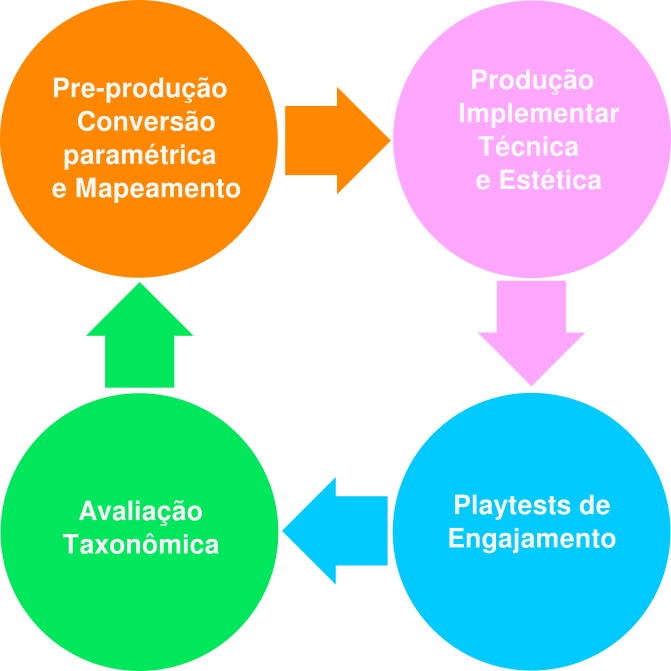
\includegraphics[width=0.4\textwidth]{images/ciclochandler.png}
    \caption{Ciclo Básico de Produção de Jogos. Fonte: adaptado de \cite{Chandler2009}.}
    \label{fig:ciclochandler}
\end{figure}


\subsection{Pré-produção e transposição didática}
A seleção dos conteúdos para o \textit{Alchemon} foi estruturada para refletir as competências de análise de fenômenos naturais da BNCC (competência EM13CNT201 da BNCC) \cite{BNCC26}, utilizando a clareza prática e experimental do currículo internacional IGCSE \cite{igcse_chemistry_2023}. 

No sistema de jogo, essa progressão curricular dita a curva de dificuldade e o desbloqueio de mecânicas:
\begin{itemize}
    \item Atomística e Tabela Periódica: Estruturam as propriedades fundamentais das criaturas (\textit{status} base de HP, ataque e defesa determinados por raio atômico e eletronegatividade).
    \item Ligações Químicas: Atuam como sistemas de sinergia em batalhas de equipe e mecânicas de evolução por fusão (combinação de elementos para formar substâncias iônicas ou covalentes).
\end{itemize}

O diferencial desta etapa reside na transformação das propriedades periódicas em regras de mecânica e atributos sistêmicos, de modo que o domínio das leis da Química se torne condição essencial para o sucesso estratégico no jogo. As mecânicas e a fundamentação teórica serão expandidas no \textit{High-Concept Document} (HCD) anexado.

\subsection{Produção e identidade visual}
A produção ocorrerá de forma iterativa, dividindo-se entre a lógica sistêmica e a construção estética. A implementação técnica das mecânicas principais e do sistema de progressão pedagógica será realizada no motor de jogos Godot \cite{Godot2024}, escolhido por sua versatilidade e sua natureza (\textit{open-source}). Em um segundo ciclo iterativo, o foco voltar-se-á para a identidade visual das criaturas, visando criar representações únicas e memoráveis para os elementos químicos.

Utilizar-se-á o \textit{software} Blender \cite{Blender2024} para modelagem 3D e o Krita \cite{Krita2024} para texturização e arte 2D. A estética será deliberadamente inspirada no estilo gráfico de \textit{Digimon World}, adotando arquétipos que facilitem a memorização visual e a conexão psicológica do jogador com sua coleção \cite{Gomez2019}. Essa abordagem visar-se-á a reduzir a carga cognitiva estranha e aumentar a curiosidade, estimulando a aprendizagem tangencial espontânea \cite{Portnow2012}.

\subsection{Testes e engajamento volitivo}
Os ciclos de testes concentrar-se-ão em usabilidade e diversão, validando se o Alchemon atenderá ao critério de ser engajador sem que a intencionalidade pedagógica prejudique o engajamento volitivo do jogador \cite{Jacobs2021}. Buscar-se-á confirmar se o jogo promove a satisfação das necessidades psicológicas básicas, especificamente autonomia e competência \cite{Ryan1985}, permitindo que o estudante sinta-se o agente de seu próprio progresso.

\section{IDENTIFICAÇÃO E RESOLUÇÃO DO PROBLEMA}

O ensino de Química, especialmente no que se refere ao domínio da Tabela Periódica, enfrenta uma persistente dificuldade de aprendizagem associada à predominância de práticas pedagógicas tradicionais baseadas na memorização mecânica, em detrimento de abordagens que promovam o engajamento ativo dos estudantes \cite{Latonio2023}. Nesse contexto, a periodicidade química é frequentemente percebida como um conteúdo abstrato e de alta complexidade, sendo abordada por meio de estratégias de memorização que não favorecem a construção de uma compreensão significativa de suas relações estruturais e funcionais \cite{Lima2010}.

Evidências empíricas demonstram a gravidade dessa lacuna, pois estudos diagnósticos revelam que estudantes de nível médio frequentemente falham em atingir o limiar básico de proficiência de 75\% em testes de compreensão da Tabela Periódica \cite{Latonio2023}. No cenário brasileiro, essa dificuldade é corroborada pelos resultados do PISA 2022, que indicam que apenas 45\% dos estudantes atingem o nível mínimo de proficiência em ciências \cite{OECD2023}.

Além das dificuldades cognitivas, a predominância de métodos expositivos e centrados no professor impacta negativamente a motivação dos estudantes e a retenção de conhecimento a longo prazo. A literatura aponta que a aprendizagem significativa está diretamente relacionada à satisfação de necessidades psicológicas básicas, como autonomia, competência e pertencimento \cite{Ryan1985}. No entanto, o modelo tradicional de ensino tende a limitar a participação ativa do estudante, o que reduz sua agência no processo de aprendizagem e contribui para o desinteresse generalizado pelos conteúdos científicos \cite{SilvaFilho2023}.

Nesse panorama, o desenvolvimento do projeto Alchemon justifica-se como uma tentativa de mitigar essas barreiras por meio de um jogo sério \cite{Plass2020}. A proposta busca converter a passividade da recepção de conteúdo em uma experiência de descoberta ativa, utilizando a estética de captura de criaturas para transformar o estudo da Química em uma ferramenta estratégica de progressão e maestria.

\subsection{Proposta de solução}
O projeto Alchemon propõe a convergência sinérgica entre a Teoria da Autodeterminação (SDT) \cite{Ryan1985}, a Aprendizagem Significativa (TAS) \cite{Ausubel1963} e a Aprendizagem Tangencial \cite{Portnow2012} para mitigar as barreiras do ensino tradicional, Fig. \ref{fig:cicloteorico}. Para evitar o fenômeno do \enquote{brócolis coberto de chocolate} \cite{Plass2020, Lorenzatti2020}, o jogo diferencia-se de abordagens educativas convencionais ao buscar uma sólida integração intrínseca (\textit{intrinsic integration}) \cite{Vahlo2023}. Assegura-se, assim, que as mecânicas lúdicas e o conteúdo científico sejam indissociáveis \cite{Plass2020}, de modo que as leis da Química não funcionem como obstáculos ou interrupções didáticas, mas constituam a própria lógica de interação e as condições de vitória do sistema \cite{Mozelius2017}.

Sob essa lógica, a solução concentra-se em satisfazer as necessidades psicológicas de autonomia e competência por meio de \textit{feedbacks} de maestria \cite{Shi2016}, transformando o conteúdo acadêmico em uma ferramenta de empoderamento estratégico \cite{Plass2020, Shi2016}. Isso garante que o jogador busque voluntariamente informações técnicas para obter vantagens \textit{in-game} \cite{Vahlo2023}, convertendo o interesse espontâneo em desempenho acadêmico mensurável \cite{LimadaCostaJunior2022}.

Para materializar esse engajamento, o projeto apoia-se na curiosidade inerente ao gênero \textit{Creature Capture} \cite{Portnow2012}, preenchendo uma lacuna teórica e estética identificada a partir dos trabalhos correlatos. Enquanto o \textit{ChemCraft} concentra-se em reações diretas e o \textit{ChemCaper} em um RPG tradicional, o Alchemon inova ao adotar uma estética de criaturas única para cada elemento químico. Superando os modelos baseados apenas em cartas ou fórmulas geométricas, essa escolha de design atua como um organizador prévio \cite{Ausubel1963}: as mecânicas de captura facilitam a memorização visual e ancoram os novos conhecimentos químicos de forma não arbitrária e substantiva, conforme os preceitos da Teoria da Aprendizagem Significativa (TAS) \cite{Ausubel1963, Espirito2020}.

Além disso, o Alchemon propõe um sistema de habilidades químicas dinâmicas baseado em propriedades periódicas, superando os modelos lineares vistos em outros trabalhos. Assim, o projeto justifica-se ao oferecer um método de estudo adaptado aos nativos digitais brasileiros, integrando as necessidades de autonomia e competência da Teoria da Autodeterminação (SDT) \cite{Ryan1985} ao ensino da Tabela Periódica no Ensino Médio.

Uma proposta incial do \textit{Game Design Document} (GDD) esta anexada\footnote{Link para o GDD http://bit.ly/43sUnRf}

\begin{figure}
    \centering
    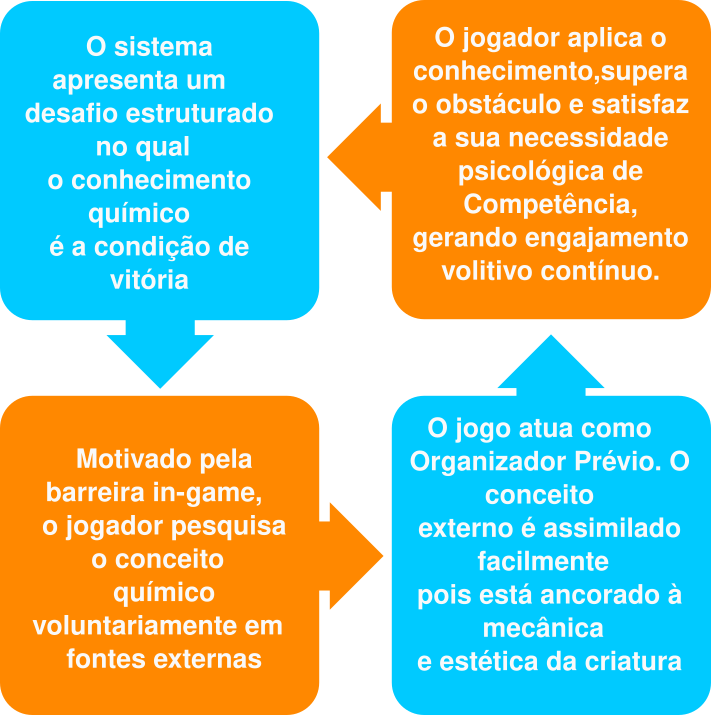
\includegraphics[width=0.4\textwidth]{images/cicloteorico.png}
    \caption{Ciclo educacional do projeto. Fonte: elaborado pelo autor.}
    \label{fig:cicloteorico}
\end{figure}

% Conclusão
\section{Conclusões Parciais e Cronograma de Trabalho}
Conclusão.

\subsection{progresso atual e viabilidade}
agora eu sabo e vai dar certo



% Impressão das referências — biblatex
\printbibliography


\end{document}


